\documentclass{article}

\usepackage[final]{neurips_2025}

\usepackage[T1]{fontenc}
\usepackage[utf8]{inputenc}
\usepackage{hyperref}
\usepackage{url}
\usepackage{booktabs}
\usepackage{amsmath,amssymb}
\usepackage{graphicx}
\usepackage{microtype}
\usepackage{subcaption}

\title{Progress Report: GFlowNet-Guided Dropout Mask Sampling for Bayesian Optimization}
\author{Anuar Aimoldin}
\date{}

\begin{document}
\maketitle

\begin{abstract}
This progress report summarizes the current status of my course project on GFlowNet-guided Bayesian optimization. The project studies whether a learned generative policy over dropout masks can improve exploration relative to random mask sampling in a neural surrogate BO loop. So far, I have implemented the full experimental pipeline, executed experiments on Branin, Hartmann-6, and Ackley-10, and written a full draft report. The current results are mixed: the learned policy underperforms random mask sampling on Branin and Hartmann-6, but improves final regret on Ackley-10. These results suggest that the approach is promising in higher-dimensional settings, but still limited by proxy-reward quality, surrogate calibration, and computational cost.
\end{abstract}

\section{Project Goal}

The project asks whether GFlowNets can be used to guide exploration in Bayesian optimization by replacing random MC-style dropout mask sampling with a learned policy. The underlying idea is that different dropout masks define different surrogate interpretations, and some of these interpretations may lead to more informative BO proposals than others. Instead of drawing masks uniformly at random, I train a sequential GFlowNet to assign higher probability to masks with larger proxy improvement potential.

\section{Progress So Far}

The main implementation work is complete. I built a reusable experiment module that contains:
\begin{itemize}
    \item benchmark definitions for Branin (2D), Hartmann-6 (6D), and Ackley (10D),
    \item a masked MLP surrogate with block-wise dropout masks,
    \item a random-mask BO baseline,
    \item a contextual sequential GFlowNet for mask generation,
    \item notebook-based evaluation and plotting utilities.
\end{itemize}

I then created and executed three separate notebooks, one for each benchmark. These notebooks compare random mask sampling and learned GFlowNet mask sampling under the same BO loop and report regret curves across five seeds. The figures from the executed notebooks were extracted and integrated into the main project report.

At a high level, the current empirical results are:
\begin{itemize}
    \item \textbf{Branin (2D):} random masks perform better than the GFlowNet policy.
    \item \textbf{Hartmann-6 (6D):} random masks again perform better.
    \item \textbf{Ackley (10D):} the GFlowNet policy performs better and reduces final regret.
\end{itemize}

This is already a meaningful result. Even though the method does not outperform the baseline everywhere, it shows a plausible dimensionality effect: learned mask generation may help more as the search problem becomes harder.

\section{Current Results}

Table~\ref{tab:progress_results} summarizes the current quantitative comparison over five seeds. The results are mixed rather than uniformly positive. On the two lower-dimensional tasks, random block-mask sampling still gives lower final regret. On Ackley-10, however, the learned GFlowNet policy reduces final regret by a noticeable margin, which is the clearest positive result so far.

\begin{table}[t]
\centering
\caption{Current final regret over 5 seeds. Lower is better.}
\label{tab:progress_results}
\small
\begin{tabular}{lcc}
\toprule
Benchmark & Random masks & GFlowNet masks \\
\midrule
Branin (2D) & $1.7813 \pm 1.1734$ & $2.1459 \pm 0.7910$ \\
Hartmann-6 (6D) & $0.5571 \pm 0.3059$ & $0.7027 \pm 0.5144$ \\
Ackley (10D) & $18.1526 \pm 1.1661$ & $16.7447 \pm 1.5421$ \\
\bottomrule
\end{tabular}
\end{table}

\begin{figure*}[t]
    \centering
    \begin{subfigure}[t]{0.32\textwidth}
        \centering
        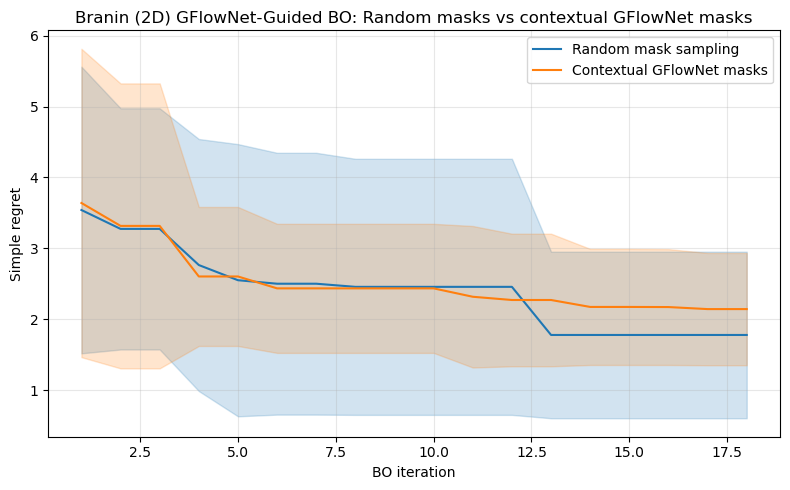
\includegraphics[width=\textwidth]{img/branin_regret_comparison.png}
        \caption{Branin (2D)}
    \end{subfigure}
    \hfill
    \begin{subfigure}[t]{0.32\textwidth}
        \centering
        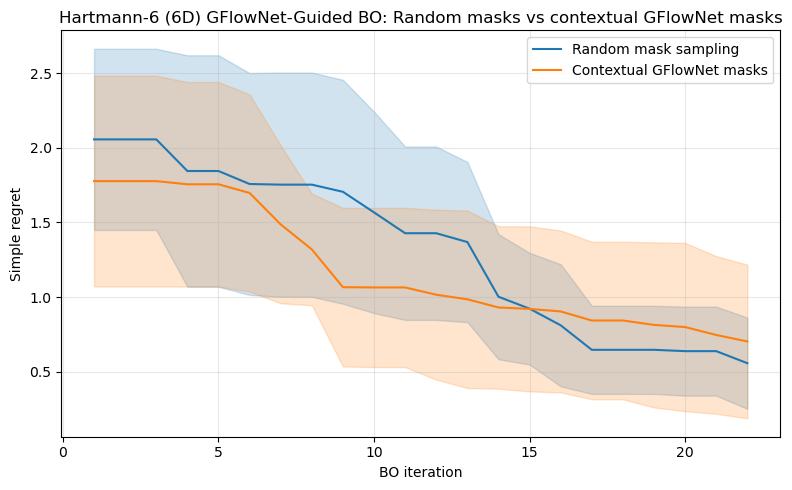
\includegraphics[width=\textwidth]{img/hartmann6_regret_comparison.png}
        \caption{Hartmann-6 (6D)}
    \end{subfigure}
    \hfill
    \begin{subfigure}[t]{0.32\textwidth}
        \centering
        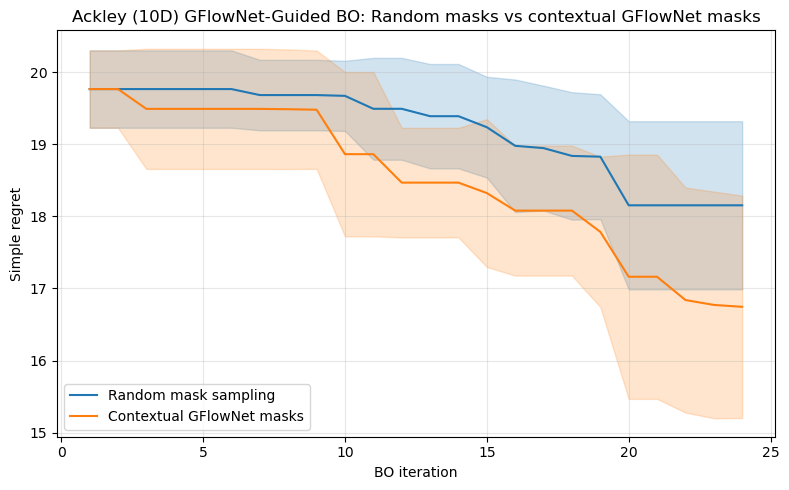
\includegraphics[width=\textwidth]{img/ackley10_regret_comparison.png}
        \caption{Ackley (10D)}
    \end{subfigure}
    \caption{Mean regret curves over BO iterations. The random baseline is stronger on Branin and Hartmann-6, while the GFlowNet policy overtakes it on Ackley-10.}
    \label{fig:progress_regrets}
\end{figure*}

Figure~\ref{fig:progress_regrets} shows the same pattern over the full optimization trajectory. The result on Ackley-10 is especially important because it suggests that learned mask generation may become more useful when the search problem is higher-dimensional and random exploration becomes weaker.

\section{Current Findings}

The strongest positive result is on Ackley-10, where the learned mask policy achieved lower mean final regret than the random baseline. This is important because Ackley is the highest-dimensional benchmark in the current suite and therefore closest to the regime where random exploration becomes weak.

At the same time, the negative results on Branin and Hartmann-6 are also informative. They suggest that the current GFlowNet objective is not yet reliably aligned with actual oracle improvement. In practice, the proxy reward can favor masks that look promising under the surrogate but do not always produce the best real BO proposals. This means that the main problem is not whether a GFlowNet can generate masks at all, but whether the reward used to train it is sufficiently well calibrated.

\section{Main Difficulties}

The biggest technical difficulty so far has been \textbf{reward design}. Since oracle evaluations are expensive, the GFlowNet is trained with a proxy reward rather than true improvement. This is necessary computationally, but it introduces a mismatch between what the GFlowNet is optimized for and what actually improves BO performance.

A second difficulty is \textbf{non-stationarity}. The mask policy is trained inside the BO loop, so the dataset and surrogate change after every query. This means that the reward landscape over masks also changes during training. I addressed this partially by conditioning the GFlowNet on simple dataset statistics, but this is only a first approximation.

A third difficulty is \textbf{computational cost}. Running the full notebooks was expensive even on these small synthetic benchmarks. The executed experiments took roughly 11 minutes for Branin, 20 minutes for Hartmann-6, and 48 minutes for Ackley-10 on my machine. This overhead is itself part of the research question, because a learned exploration policy is only useful if the extra training cost is justified by better sample efficiency.

\section{Next Steps}

The next stage of the project will focus on improving the method rather than only extending the benchmark list.

\begin{itemize}
    \item \textbf{Improve reward quality:} test alternative proxy rewards, including more conservative uncertainty-aware rewards and held-out surrogate checks.
    \item \textbf{Handle non-stationarity better:} compare continual fine-tuning with periodic retraining and improve the context representation given to the GFlowNet.
    \item \textbf{Strengthen evaluation:} run additional seeds and test whether the Ackley improvement is robust.
    \item \textbf{Compare compute vs.\ benefit:} explicitly measure whether regret reduction is worth the extra optimization cost.
    \item \textbf{Optional baselines:} if time permits, compare with other uncertainty-aware neural BO approaches such as deep ensembles or concrete dropout.
\end{itemize}

\section{Conclusion}

The project is in a good proof-of-concept stage. The full pipeline is implemented, the required benchmark experiments have been executed, and the report draft has been updated with real results and plots. The current evidence does not show that GFlowNet-guided mask generation is universally better than random mask sampling, but it does show one encouraging success case on Ackley-10. This is enough to support a focused final stage centered on reward improvement, non-stationarity handling, and a clearer computational trade-off analysis.

\bibliographystyle{plainnat}
\bibliography{references}

\end{document}
